
%(BEGIN_QUESTION)
% Copyright 2010, Tony R. Kuphaldt, released under the Creative Commons Attribution License (v 1.0)
% This means you may do almost anything with this work of mine, so long as you give me proper credit

A safety device commonly installed on process vessels containing pressurized gases is a {\it Pressure Safety Valve}, or PSV.  In this example, a PSV protects a storage tank against rupture from excessive internal gas pressure, with the PSV set to open (``lift'') and vent the tank if the internal pressure exceeds 2 inches water column:

$$\includegraphics[width=15.5cm]{i03590x01.eps}$$

Calculate the total upward force exerted on the circular roof of this cylindrical storage tank at the PSV lift pressure, expressed in the unit of {\it tons}.

\vskip 10pt

$F$ = \underbar{\hskip 50pt} tons

\vfil 

\underbar{file i03590}
\eject
%(END_QUESTION)





%(BEGIN_ANSWER)

This is a graded question -- no answers or hints given!
 
%(END_ANSWER)





%(BEGIN_NOTES)

The general principle to apply here is the relationship between pressure, surface area, and force ($F = PA$).  We will need to convert units in order to have the variables $P$ and $A$ appropriately scaled for use in this formula (PSI and square inches, respectively), then convert the resulting force ($F$) figure of pounds into the final unit of tons.  

Since the area of the roof ($A$) is not given to us in the problem, we will need to calculate it somehow based on the given tank dimensions.  We know that circular objects have areas equal to $A = \pi r^2$, so what we can do here is take the tank's diameter of 30 feet and divide by 2 to get the radius, then calculate area from that.  A radius of 15 feet is equal to a radius of 180 inches.  Squaring 180 inches and multiplying by $\pi$ yields an area of 101,787.6 square inches.

\vskip 10pt

A useful strategy to apply in {\it any} physics formula is to express all the units of measurement, and then see how the units cancel to yield the answer.

\vskip 10pt

2 inches WC = 0.072254 PSI

30 feet diameter roof = 101,787.6 square inches of area

$$F = PA = \left( 0.072254 \hbox{ lb} \over \hbox{in}^2 \right) \left( 101787.6 \hbox{ in}^2 \right)$$

$$F = 7,354.6 \hbox{ pounds} = 3.6773 \hbox{ tons}$$

%INDEX% Physics, fluids: pressure, force, and area
%INDEX% Physics, units and conversions: pressure
%INDEX% Safety, overpressure protection: safety valve

%(END_NOTES)


